\documentclass[11pt, oneside]{article}   	% use "amsart" instead of "article" for AMSLaTeX format
\usepackage{amssymb}
\usepackage{commath}
\usepackage{physics}
\usepackage{tikz,tikz-3dplot}
% --------------------------------------- Title Matter -----------------------------------------

\title{Derivation of the Differential Continuity Equation}
\author{Eric Mott}
\date{2015-10-11}					% Activate to display a given date or no date

% --------------------------------------- Begin Document -----------------------------------------

\begin{document}
\maketitle 							% Places title matter

% --------------------------------------- Section 2 -----------------------------------------

\section{Continuity Equation}			% Creates a numbered section

\begin{figure}
\centering
\tdplotsetmaincoords{305}{75}
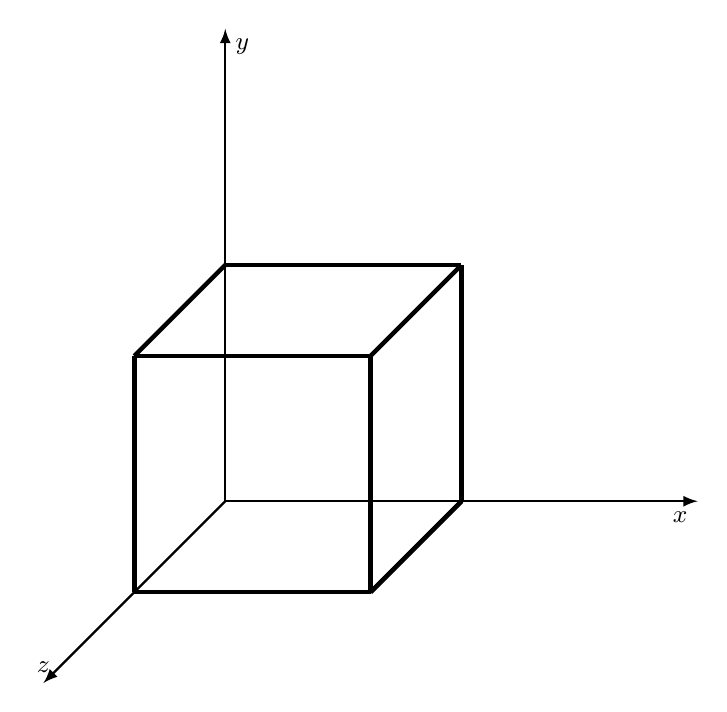
\begin{tikzpicture}[scale=3]
\tikzstyle{every node}=[font=\small]
\draw[thick,-latex] (0,0,0) -- (2,0,0) node[anchor=north east]{$x$};
\draw[thick,-latex] (0,0,0) -- (0,2,0) node[anchor=north west]{$y$};
\draw[thick,-latex] (0,0,0) -- (0,0,2) node[anchor=south]{$z$};
\draw [ultra thick] (0,1,1)--(0,1,0);
\draw [ultra thick] (0,1,0)--(1,1,0);
\draw [ultra thick] (1,1,1)--(1,1,0);
\draw [ultra thick] (1,1,1)--(1,0,1);
\draw [ultra thick] (1,1,1)--(0,1,1);
\draw [ultra thick] (1,1,0)--(1,0,0); 
\draw [ultra thick] (1,0,0)--(1,0,1);
\draw [ultra thick] (1,0,1)--(0,0,1);
\draw [ultra thick] (0,1,1)--(0,0,1);

\draw [ultra thick] (1,0,1)--(1,0,0);

\end{tikzpicture}
\end{figure}

Starting with the first principle of conservation of mass:

\begin{equation}
\text{time rate change in mass} = \text{mass transfer in} - \text{mass transfer out}
\end{equation}

\noindent 
This can be expressed mathematically as:

\begin{equation}
\pdv{m}{t} = \dot{m}_{in} - \dot{m}_{out}
\end{equation}

\begin{equation}
\pdv{m}{t} = (\rho A u)_{in} - (\rho A u)_{out}
\end{equation}

\noindent
For the infinitesimal control volume defined by lengths $\dif x$, $\dif y$, and $\dif z$, mass can be expressed in terms of the density, $\rho$, as:

\begin{equation}
m = \rho \dif x \dif y \dif z
\end{equation}

\begin{equation}
\pdv{\rho}{t} \dif x \dif y \dif z = \dot{m}_{in} - \dot{m}_{out}
\end{equation}

\begin{equation}
\frac{\Dif \rho}{\Dif t}   = - \rho \div \vec{u}
\end{equation}

\end{document}